% Fonte tamanho 11, duas colunas, tipo artigo.
\documentclass[11pt, article]{article}

% Escrita em português
\usepackage[utf8]{inputenc}
\usepackage[T1]{fontenc}
\usepackage[portuges, english]{babel}

% Inclusão de Imagens
\usepackage{graphicx}
% \usepackage[outdir=./]{epstopdf}
% Para incluir imagens usando o ambiente figure*, cuja vantagem é
% a possibilidade de inclusão de imagens que ocupam as 2 colunas,
% além de incluir duas figuras lado a lado, use a sintaxe:
        % \begin(figure*)[!htp]
        %         \centering
        %         \includegraphics[width=0.45\linewidth]
        %                         {imagem_1.png}
        %         \includegraphics[width=0.45\linewidth]
        %                         {imagem_2.png}
        %         \caption{\small Descrição das figuras.}
        %         \label{REFERENCIA_FIGURA_ASTERISCO}
        % \end{figure*}
% Os termos [!htp] servem para sinalizar a posição da figura e
% forçá-la em determinada posição. Em geral são suficientes.
% Para uma figura de uma única coluna, o ambiente figure pode ser
% usado da seguinte forma:
        % \begin(figure)[htp]
                % \centering
                % \includegraphics[width=0.9\linewidth]
                %                 {imagem.png}
                % \caption{\small Descrição das figuras.}
                % \label{REFERENCIA_FIGURA}
        % \end{figure}

% Correção de Margens
\usepackage
[
        top = 2.5cm,
        left = 2.5cm,
        right = 2.5cm,
        bottom = 2.5cm
]{geometry}

% Símbolos Matemáticos
\usepackage{amsmath}
\usepackage{mathrsfs}
% Altera sin(x) para sen(x)
\def\sen{\mathop{\mbox{\normalfont sen}}\nolimits}
% O pacote amsmath dá acesso ao ambiente equation*, que não numera
% as equações, diferente do ambiente equation. Para usá-los,
% a sintaxe utilizada é:
        % \begin{equation}
        %         \sigma_{\overline{x}} =
        %                 \sqrt{
        %                         \frac
        %                         {
        %                                 \sum_{i = 1}^{n}
        %                                 \delta_{i}^{2}
        %                         }
        %                         {
        %                                 n(n - 1)
        %                         }
        %                 }
        % \end{equation}
        %
        % \begin{equation*}
        %         \sigma_{\overline{x}} =
        %                 \sqrt{
        %                         \frac
        %                         {
        %                                 \sum_{i = 1}^{n}
        %                                 \delta_{i}^{2}
        %                         }
        %                         {
        %                                 n(n - 1)
        %                         }
        %                 }
        % \end{equation*}


% Unidades do SI
\usepackage{siunitx}
% Para usar a unidade do SI, escreva da seguinte forma, por
% exemplo, para 10 metros:
        % \SI{10}{\metre}

% Tabelas
\usepackage{booktabs}
\usepackage{array}
\usepackage{multirow}
\usepackage{multicol}
% Esses pacotes possibilitam maior flexibilidade na construção de
% tabelas. Um exemplo de tabela pode ter a forma:
                % \begin{table}[!htp]
                %         \begin{tabular}{m{0.225\linewidth}
                %                         m{0.225\linewidth}
                %                         m{0.225\linewidth} c}
                %                         \toprule
                %                 % Nome das Colunas
                %                 Grandeza &
                %                 \hbox{Valor} Teórico &
                %                 \hbox{Valor} Prático & Desvio\\
                %                 \midrule
                %
                %                 % Linha 1
                %                 $f$ (\SI{}{\hertz}) &
                %                 60,00 &
                %                 60,10 &
                %                 0,17\% \\
                %
                %                 % Linha 2
                %                 $V_{L}$ (\SI{}{\volt}) &
                %                 30,00 &
                %                 29,28 &
                %                 2,42\% \\
                %
                %                 % Linha 3
                %                 $I_{L}$ (\SI{}{m\ampere}) &
                %                 \SI{300,0}{} &
                %                 \SI{290,0}{} &
                %                 3,42\% \\
                %
                %                 % Linha 4
                %                 $\phi$ (\SI{}{\radian}) &
                %                 0.00 &
                %                 0,00 &
                %                 0,00\% \\ \hline
                %         \end{tabular}
                %         \caption{\small Descrição da tabela}
                %         \label{REFERENCIA_TABELA}
                % \end{table}
% Assim como nas figuras, os parâmetros [!htp] servem para ajuste
% de posição. Mais formas de tabela pode ser vistos em:
% https://en.wikibooks.org/wiki/LaTeX/Tables

% Bibliografia
\usepackage
[
        % IEEE parece ter o estilo mais próximo
        style     = ieee,
        citestyle = numeric
]{biblatex}
% Referências para o uso desse pacote podem ser encontradas em:
% www.sharelatex.com/learn/Bibliography_management_with_biblatex
\bibliography{bibliography.bib}


% Pacotes de rascunho
\usepackage{lipsum}

% Macro para valores com variação
\newcommand{\val}[1]{\num[separate-uncertainty]{#1}}
% Uso: \val{9.787604(9)E+0}

% Variáveis de informação
% Título
\newcommand{\vartitulo}{Título do Relatório}
% Nome (Formato A. B. C. Sobrenome)
\newcommand{\varautor}{A. B. C. Sobrenome}
% Instituição de Ensino
\newcommand{\varinstituicao}{Universidade Universidade}
% Departamento
\newcommand{\vardepartamento}{Departamento de Departamento}
% Informações de contato
\newcommand{\varcontato}{Caixa Postal: XXXXX -
                         CEP: XXXXX-XXX -
                         Cidade -
                         Estado \\
                         Fone: +XX-XX-XXXX-XXXX -
                         Fax: +XX-XX-XXXX-XXXX \\
                         email@de.contato}

% Informações para o título
\title{\vartitulo}
\author
{
        \varautor \\
        \varinstituicao \\
        \vardepartamento \\
        \varcontato
}
\date{}

\begin{document}

        \paragraph{}
	\begin{tabular}{c ccc}
        \hline
                      & \multicolumn{3}{c}{Método} \\ \cline{2-4}
        Nota de corte & Média com BD & Média sem BD & Independentes \\
        \hline
        0    & 7.2     & 7.50143  & 7.54987 \\
        0.2  & 7.2     & 7.37301  & 7.84565 \\
        1.1  & 7.2     & 7.23458 & 7.74893  \\
        3    & 7.08109 & 7.08109 & 7.53332  \\
        3.2  & 6.73897 & 6.73897 & 7.24801  \\
        6.1  & 6.60445 & 6.60445 & 7.28547  \\
        6.3  & 6.53667 & 6.48256 & 7.0332   \\
        7.1  & 6.53667 & 6.30198 & 6.37349  \\
        8.5  & 6.53667 & 6.32048 & 6.18549  \\
        8.8  & 6.53667 & 6.41722 & 6.5049   \\
        9.3  & 6.53667 & 6.46296 & 6.14667  \\
        9.6  & 6.53667 & 6.53667 &          \\
        \hline
\end{tabular}
 \\[30pt]
        \paragraph{}
	\begin{tabular}{c cccc}
        \hline
                      & \multicolumn{4}{c}{Pesos}\\ \cline{2-5}
        Nota de corte & Prova 1  & Prova 2 & Relatório 1
        & Relatório 2 \\
        \hline
        0    & 0.1386   & -0.414789  & 0.822417  & 0.453772  \\
        0.2  & 1.14185  & -0.744971  & -0.347389 & 0.950513  \\
        1.1  & 1.66639  & -0.756088  & -0.735138 & 0.824836  \\
        3    & 1.31196  & -0.437053  & -0.805813 & 0.93091   \\
        3.2  & 1.10159  & -0.135964  & -0.754942 & 0.789316  \\
        6.1  & 1.5482   & -0.304536  & -0.826339 & 0.582674  \\
        6.3  & 1.32118  & -0.0287221 & -0.761471 & 0.469017  \\
        7.1  & 0.672257 & 0.661219   & -0.368195 & 0.0347192 \\
        8.5  & 0.42029  & 0.86087    & -0.167391 & -0.113768 \\
        8.8  & 0.678161 & 0.448276   & 0.0775862 & -0.204023 \\
        9.3  & 0        & 1          & 0         & 0         \\
        \hline
\end{tabular}
 \\[30pt]
        \paragraph{}
	\begin{tabular}{c cccc}
        \hline
                      & \multicolumn{2}{c}{Pesos com BD}
                      & \multicolumn{2}{c}{Pesos sem BD} \\ \cline{2-5}
        Nota de corte & Provas & Relatórios & Provas & Relatórios \\
        \hline
        0    & 0        & 1        & -0.454422 & 1.45442    \\
        0.2  & 0        & 1        & -0.260823 & 1.26082    \\
        1.1  & 0        & 1        & -0.052136 & 1.05214    \\
        3    & 0.179256 & 0.820744 & 0.179256  & 0.820744   \\
        3.2  & 0.695018 & 0.304982 & 0.695018  & 0.304982   \\
        6.1  & 0.897815 & 0.102185 & 0.897815  & 0.102185   \\
        6.3  & 1        & 0        & 1.08157   & -0.0815747 \\
        7.1  & 1        & 0        & 1.3538    & -0.353799  \\
        8.5  & 1        & 0        & 1.32591   & -0.325905  \\
        8.8  & 1        & 0        & 1.18008   & -0.180077  \\
        9.3  & 1        & 0        & 1.11111   & -0.111111  \\
        9.6  & 1        & 0        & 1         & 0          \\
        \hline
\end{tabular}
 \\[30pt]
        \paragraph{}
	\begin{tabular}{c ccc ccc ccc}
        \hline
                      & \multicolumn{3}{c}{Médio com BD}
                      & \multicolumn{3}{c}{Médio sem BD}
                      & \multicolumn{3}{c}{Independentes} \\
                      \cline{2-10}
        Nota de corte & Apr. & Final & Rep.
                      & Apr. & Final & Rep.
                      & Apr. & Final & Rep. \\
        \hline
        0    & 13 & 1 & 1    & 10 & 5 & 0    & 11 & 4 & 0 \\
        0.2  & 13 & 1 & 1    & 10 & 5 & 0    & 12 & 2 & 1 \\
        1.1  & 13 & 1 & 1    &  9 & 5 & 1    & 11 & 3 & 1 \\
        3    & 11 & 3 & 1    & 11 & 3 & 1    & 11 & 2 & 2 \\
        3.2  &  9 & 4 & 2    &  9 & 4 & 2    & 11 & 2 & 2 \\
        6.1  &  9 & 2 & 4    &  9 & 2 & 4    & 10 & 3 & 2 \\
        6.3  &  9 & 2 & 4    &  7 & 4 & 4    & 10 & 3 & 2 \\
        7.1  &  9 & 2 & 4    &  7 & 4 & 4    &  9 & 2 & 4 \\
        8.5  &  9 & 2 & 4    &  7 & 4 & 4    &  7 & 4 & 4 \\
        8.8  &  9 & 2 & 4    &  7 & 4 & 4    &  7 & 4 & 4 \\
        9.3  &  9 & 2 & 4    &  7 & 4 & 4    &  7 & 4 & 4 \\
        9.6  &  9 & 2 & 4    &  9 & 2 & 4    &    &   &   \\
        \hline
\end{tabular}
 \\[30pt]


        \begin{figure}[!htb]
                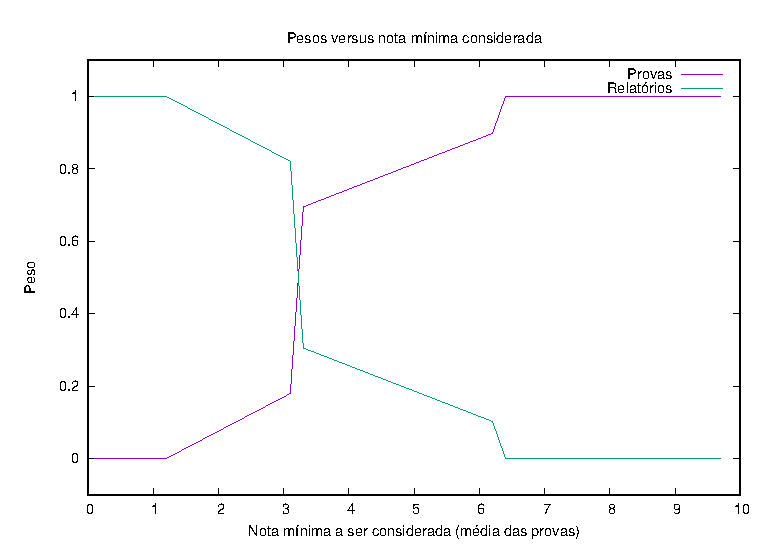
\includegraphics
                [width=0.85\linewidth]
                {./img/media_bd/weights.eps}
        \end{figure}
        \begin{figure}[!htb]
                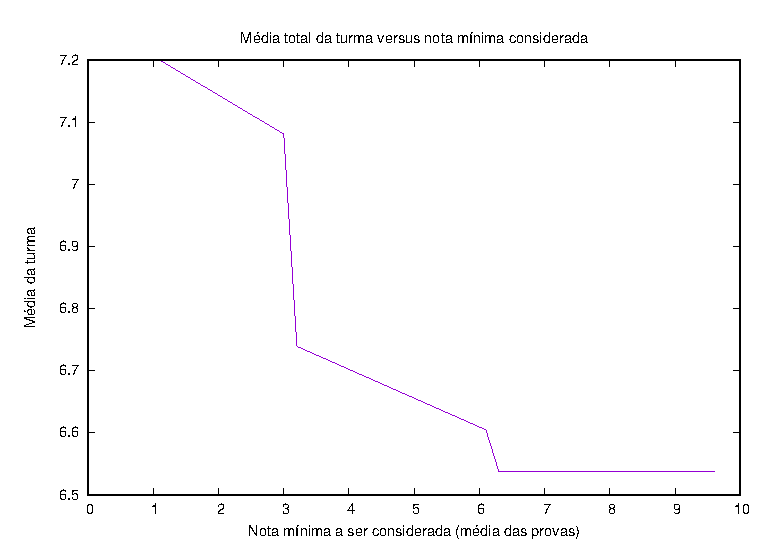
\includegraphics
                [width=0.85\linewidth]
                {./img/media_bd/total_class_average.eps}
        \end{figure}
        \begin{figure}[!htb]
                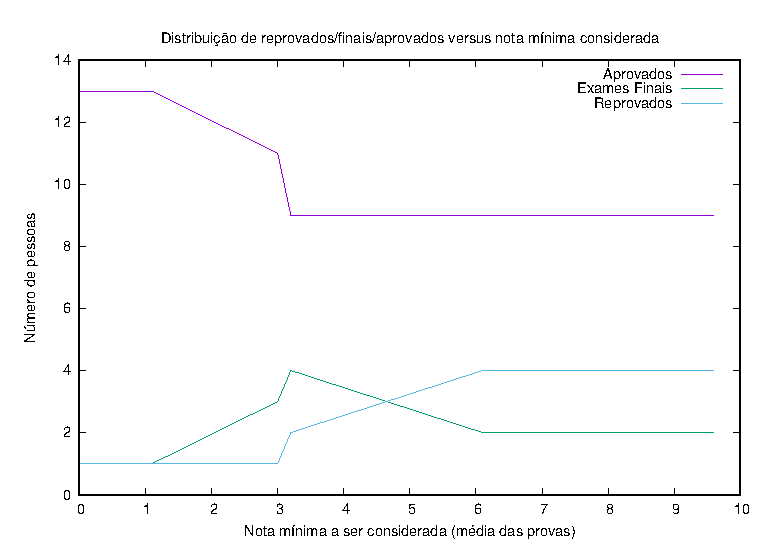
\includegraphics
                [width=0.85\linewidth]
                {./img/media_bd/final_state.eps}
        \end{figure}

        \begin{figure}[!htb]
                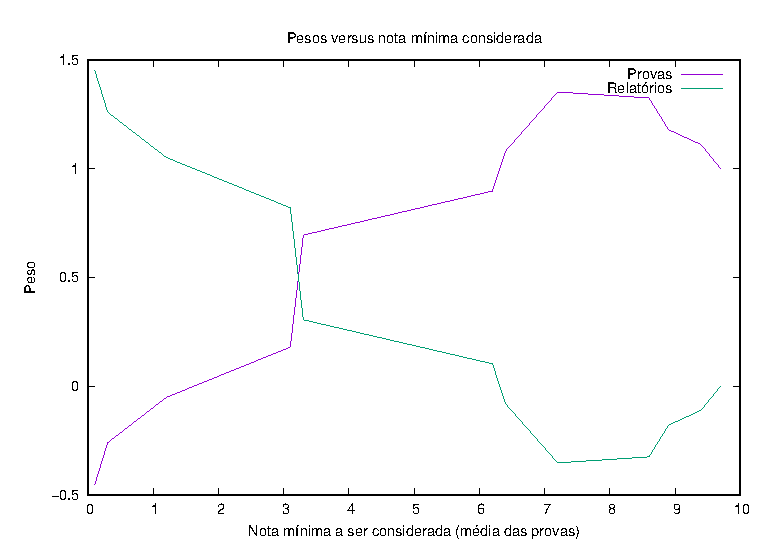
\includegraphics
                [width=0.85\linewidth]
                {./img/media_sem_bd/weights.eps}
        \end{figure}
        \begin{figure}[!htb]
                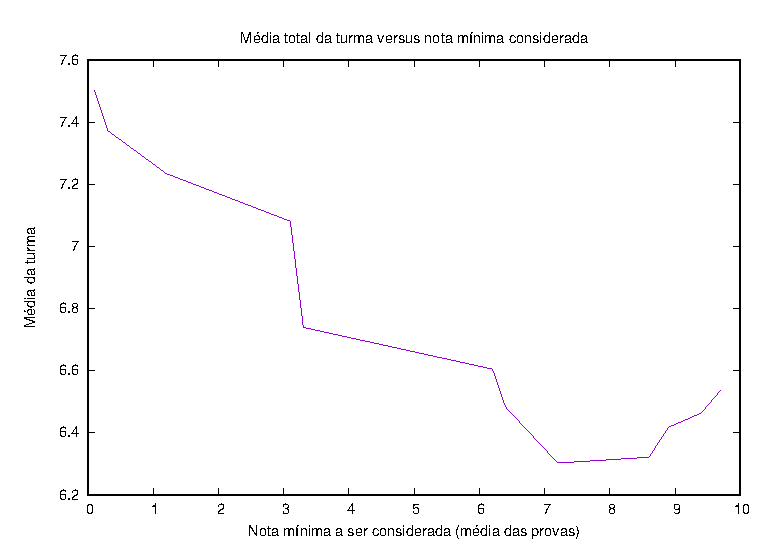
\includegraphics
                [width=0.85\linewidth]
                {./img/media_sem_bd/total_class_average.eps}
        \end{figure}
        \begin{figure}[!htb]
                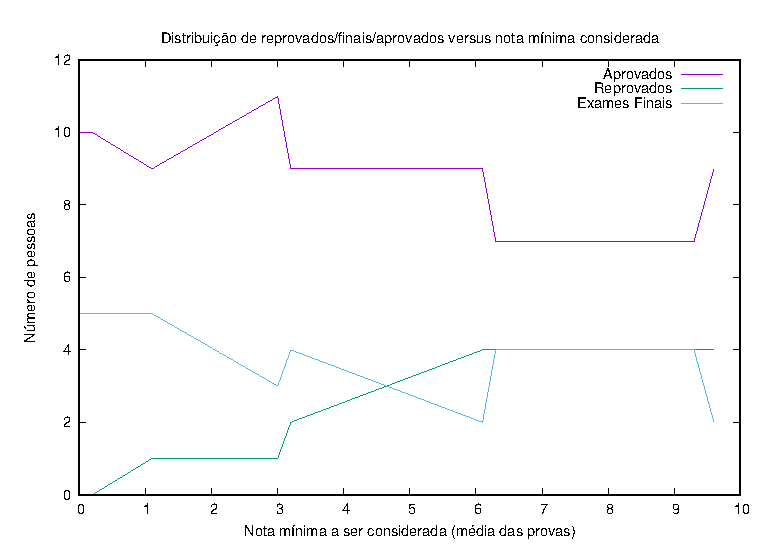
\includegraphics
                [width=0.85\linewidth]
                {./img/media_sem_bd/final_state.eps}
        \end{figure}

        \begin{figure}[!htb]
                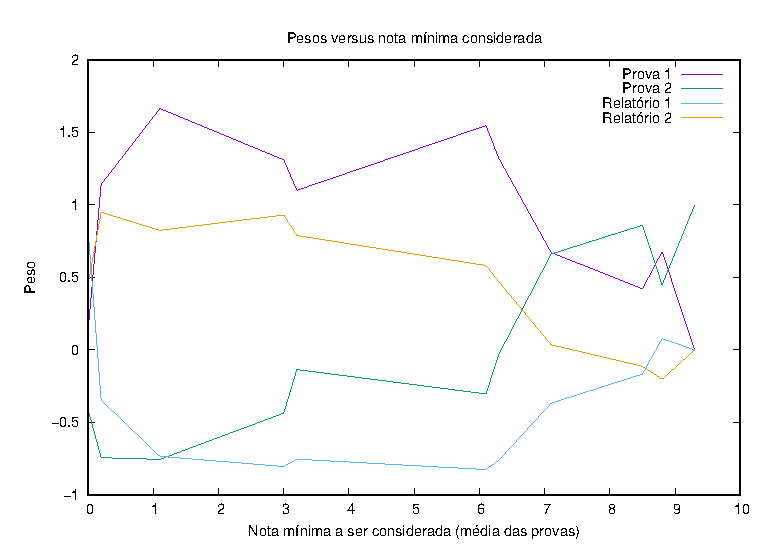
\includegraphics
                [width=0.85\linewidth]
                {./img/independente/weights.eps}
        \end{figure}
        \begin{figure}[!htb]
                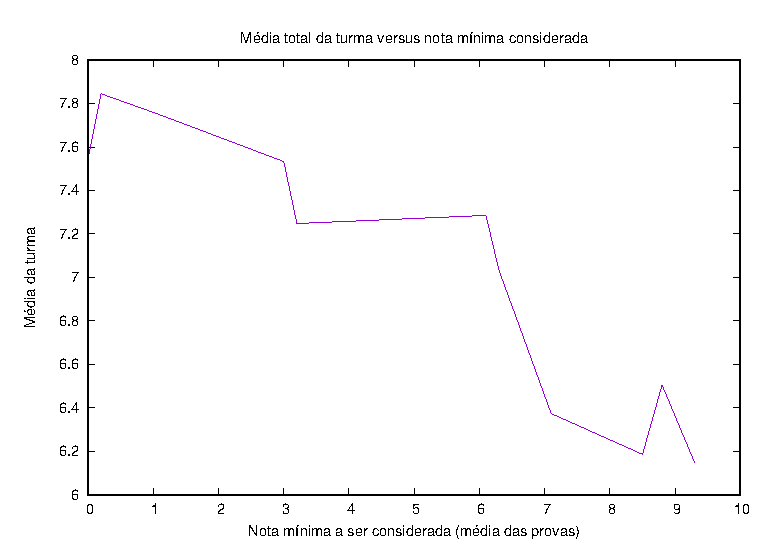
\includegraphics
                [width=0.85\linewidth]
                {./img/independente/total_class_average.eps}
        \end{figure}
        \begin{figure}[!htb]
                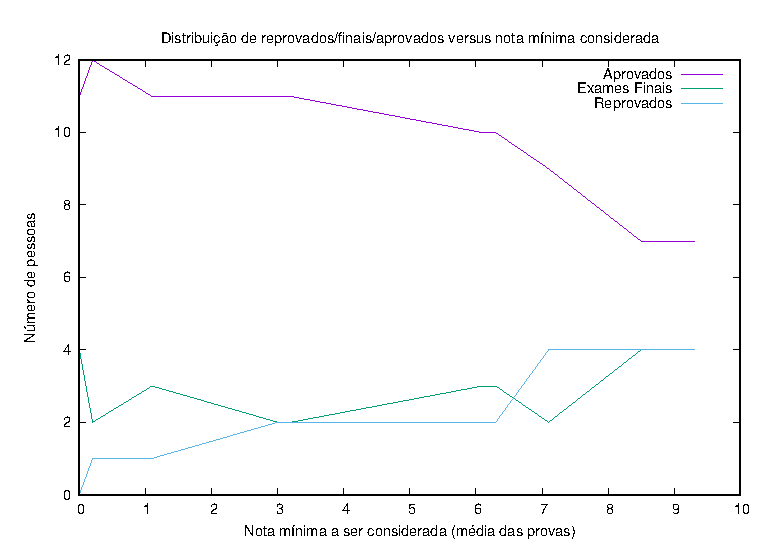
\includegraphics
                [width=0.85\linewidth]
                {./img/independente/final_state.eps}
        \end{figure}


\end{document}
